\chapter{Hypothesis Testing and Model Selection}
Hypothesis testing (also known as model selection, particularly when it is
done using the method in Section~\ref{sec:marginal_likelihood})
is a very important topic that is traditionally considered
as a different topic from parameter estimation. However, in Bayesian statistics
we will see that hypothesis testing is basically the same thing as parameter
estimation! The one difference, for us, will be that we will sometimes change
the prior distribution a little bit.

One big advantage of Bayesian statistics is that it {\it unifies}
parameter estimation and hypothesis
testing\footnote{``Unifies'' is a popular word for physicists. It means that
two seemingly different topics are fundamentally the same, or at least closely
related.}. That's good news, because it means that instead of having to
understand two different topics, we only have to understand one!

To see why hypothesis testing is fundamentally the same as parameter estimation,
you only need to
understand how parameter estimation works from a Bayesian point of view, which
we have already studied.
Parameter estimation is nothing more than testing a bunch of hypotheses about
the value of the parameter! e.g. $\theta=1$ vs. $\theta=2$ vs. $\theta=3$ and
so on. If we have their posterior probabilities, then we've tested them.

\section{An Example Hypothesis Test}
Suppose we were performing a Bayesian parameter estimation analysis using a
Bayes' Box. Here is an example Bayes' Box with made up numbers:

\begin{table}[h!]
\begin{center}
\begin{tabular}{|c|c|c|c|c|}
\hline
\tt{possible values} & \tt{prior} & \tt{likelihood} & \tt{prior} $\times$ \tt{likelihood} & \tt{posterior}\\
$\theta$ & $p(\theta)$ & $p(x|\theta)$ & $p(\theta)p(x|\theta)$ & $p(\theta|x)$\\
\hline
1.5 & 0.25 & 0.2 & 0.05 & 0.1\\
2.0 & 0.25 & 0.4 & 0.1 & 0.2\\
2.5 & 0.25 & 0.6 & 0.15 & 0.3\\
3.0 & 0.25 & 0.8 & 0.2 & 0.4\\
\hline
Totals & 1 & & 0.5 & 1\\
\hline
\end{tabular}
\end{center}
\end{table}
Suppose we wanted to test the following two hypotheses about the parameter $\theta$.
The first hypothesis $H_0$ is a ``null hypothesis'', and the second hypothesis,
$H_1$, is an ``alternative hypothesis''.
\begin{eqnarray}
H_0: && \theta = 2\\
H_1: && \theta \neq 2
\end{eqnarray}
In classical statistics, if you saw a question phrased in this way, you would
need to come up with a {\it test statistic},
and then calculate a {\it p-value} which tries to say something about whether
the value of the test statistic would be considered extreme, under the
assumption that $H_0$ is true.
In Bayesian statistics, the only thing we need to do is calculate
the posterior probability of $H_0$ and the posterior probability of $H_1$.
The posterior probability of $H_0$ is given by:
\begin{eqnarray}
P(H_0|x) &=& P(\theta = 2|x)\\
&=& 0.2
\end{eqnarray}
All we did here was look up the appropriate number in the Bayes' Box! The
posterior probability of $H_1$ is only slightly harder (but still easy)
to calculate: $H_1$ will
be true if $\theta$ takes any value other than 2. Therefore the posterior
probability of $H_1$ is
\begin{eqnarray}
P(H_1|x) &=& P(\theta = 1.5 \textbf{ or } \theta = 2.5 \textbf{ or } \theta = 3|x)\\
&=& P(\theta = 1.5|x) + P(\theta = 2.5|x) + P(\theta = 3|x)\\
&=& 0.1 + 0.3 + 0.4\\
&=& 0.8.
\end{eqnarray}
Here we used the fact that everything in a Bayes' Box is mutually exclusive
(only one of the hypotheses is true) so we could add the probabilities.
Alternatively, you could have just noticed that $H_1$ is true if $H_0$ is false.
So $P(H_0|x) + P(H_1|x) = 1$, which implies $P(H_1|x) = 1 - P(H_0|x)$.

\section{The ``Testing'' Prior}
Here we will study a hypothesis testing example that involves a null and an
alternative hypothesis. Since the bus example has been used a lot, we will now
switch over to a different example.

Suppose it is known that the mean systolic blood pressure
in the general population is 120 mm Hg, with a standard deviation of
15 mm Hg (millimetres of mercury is an
old fashioned unit for pressure, even though it sounds like a unit of length).
A new drug is developed that may
be helpful in reducing blood pressure. A sample of 100 people
(that can be considered representative of the general population)
are given the drug, and their systolic blood pressure is measured. This results
in 100 blood pressure measurements $\{x_1, x_2, ..., x_{100}\}$, which will be
our data.

We are interested in whether the drug works. Let $\mu$ be the mean systolic
blood pressure
that would apply in the general population if everyone was taking the
drug. Our goal is to infer the value of $\mu$ from the data. In classical
statistics, this is sometimes phrased as a hypothesis test between the two
competing hypotheses. We will not be concerned with the possibility that the
drug has the opposite effect to what is intended.
\begin{equation}
\begin{array}{ll}
H_0: & \mu = 120 \textnormal{ (the drug does nothing)}\\
H_1: & \mu < 120 \textnormal{ (the drug reduces blood pressure)}
\end{array}
\end{equation}
Suppose the mean of all the data values was
\begin{eqnarray}
\bar{x} &=& \frac{1}{N} \sum_{i=1}^{100} x_i\\
&=& 115.9.
\end{eqnarray}
Does this data provide evidence against $H_0$ and in favour of $H_1$? In
classical statistics this question would be addressed using a {\it p-value}.
The p-value would be the probability of getting a result this extreme or
a result more extreme than what is observed, assuming that the ``null hypothesis''
is true. That is,
\begin{eqnarray}
\textnormal{p-value} = P(\bar{x} \leq 115.9 | H_0).
\end{eqnarray}
In case you're curious, the p-value in this case is 0.0031, which is usually
taken to mean that there is fairly strong evidence against $H_0$ and in favour
of $H_1$. To calculate the p-value I had to assume that the probability distribution
for the data values $\{x_1, x_2, ..., x_{100}\}$ was a normal distribution
with a known standard deviation of $\sigma=15$, and
that they were independent:
\begin{eqnarray}
x_i \sim \mathcal{N}(\mu, \sigma^2). \label{eq:normal}
\end{eqnarray}

In Bayesian statistics, p-values are not used. Instead, we should think of this
as a parameter estimation problem. We can state a set of hypotheses about the
value of $\mu$, and then choose a prior distribution, update to a posterior
distribution, etc. Then we will end up with the posterior probability of the
null hypothesis, $P(H_0 | \{x_1, ..., x_{100}\}) = P(\mu = 120 | \{x_1, ..., x_{100}\})$.
This is great, because the posterior probability of the null hypothesis is
exactly what we want. It is a description of how plausible the null hypothesis
is, given the data. It is not some other probability that isn't really relevant.
We can also get the posterior probability of $H_1$ by summing the posterior
probabilities for all other values of $\mu$ apart from 120, or by using
$P(H_1 | \{x_1,...,x_{100}\}) = 1 - P(H_0 | \{x_1,...,x_{100}\})$.

There is only one minor tweak we need to make to make Bayesian inference an
appropriate framework for solving this problem. When the null and alternative
hypotheses are written like we did above, it implies that the value of $\mu$
that we are calling the ``null hypothesis'' is a {\it special value that is
especially plausible}. To take this into account in our Bayesian analysis we
need to make sure that the prior distribution recognises that there is a special
value of the parameter that we think is extra plausible. When we do this, we
will call it a {\it testing prior}. An example of a testing prior, and the
resulting Bayes' Box, for
the blood pressure problem is given in Table~\ref{tab:testing_prior}.
The R code for calculating these results is given below.

\begin{framed}
\begin{verbatim}
# Parameter values
mu = seq(110, 120)

# Make the testing prior
prior = rep(0.5/10, 11)
prior[11] = 0.5

# Compute the likelihood for the 100 data points.
# The numbers get close to 0, so logs would be useful
lik = 1
# Use a for loop to loop over all data values
# and multiply the likelihoods
for(i in 1:100)
{
    lik = lik*dnorm(x[i], mean=mu, sd=15)
}

# Rescale the likelihood for readability
lik = lik/max(lik)*1000

# Calculate the posterior
h = prior*lik
post = h/sum(h)

# The null hypothesis
post[11]
\end{verbatim}
\end{framed}


\begin{table}[ht!]
\begin{center}
\begin{tabular}{|c|c|c|c|c|}
\hline
\tt{possible values} & \tt{prior} & \tt{likelihood} & \tt{prior} $\times$ \tt{likelihood} & \tt{posterior}\\
$\mu$ & $p(\mu)$ & $p(\{x_1, ..., x_{100}\}|\mu)$ & $p(\mu)p(\{x_1, ..., x_{100}\}|\mu)$ & $p(\mu|\{x_1, ..., x_{100}\})$\\
\hline
110 & 0.05 & 0.44	& 0.02 & 0.0001\\
111 & 0.05 & 4.83	& 0.24 & 0.0012\\
112 & 0.05 & 34.12	& 1.71 & 0.0086\\
113 & 0.05 & 154.64	& 7.73 & 0.0389\\
114 & 0.05 & 449.33	& 22.47 & 0.1129\\
115 & 0.05 & 837.13	& 41.86 & 0.2103\\
116 & 0.05 & 1000.00    & 50.00 & 0.2512\\
117 & 0.05 & 756.93	& 38.30 & 0.1924\\
118 & 0.05 & 376.15	& 18.81 & 0.0945\\
119 & 0.05 & 118.44	& 5.92 & 0.0298\\
{\bf 120} & {\bf 0.5}   & {\bf 23.91} & {\bf 11.96} & {\bf 0.0601}\\
\hline
Totals & 1 & & 630.3036 & 1\\
\hline
\end{tabular}
\caption{\it An example of a testing prior for the blood pressure problem. We
give more prior probability to the special value $\mu=120$ because it is
particularly plausible. For readability I have rescaled the likelihoods so that
the maximum is 1000. Note that the posterior probability of $H_0$ can simply
be read off the table.
\label{tab:testing_prior}}
\end{center}
\end{table}

In Figure~\ref{fig:testing_priors}, there are three possible ideas for priors
for the blood pressure question. They all may seem reasonable in this situation.
Prior 1 is basically the same as the prior in our Bayes' Box, although it goes
down to $\mu=100$ and divides the possible $\mu$ values more finely. This prior
says the null has a 50\% probability, and if $\mu$ is not equal to 120 then it
could be anything.
Prior 2
is similar but has only 30\% of the prior probability on the null hypothesis
instead of 50\%,
and the shape of the prior is non-uniform for the lower values of $\mu$.
This is like saying ``$\mu$ could be precisely 120, and if it's not precisely
120 then it is probably at least {\it close} to 120''.
Prior 3 isn't really a testing prior at all (it doesn't have a spike), but is
just a bell-shaped prior. This is like saying ``alright, I would never believe
$\mu$ is {\it exactly} 120, but I think there's a reasonable chance it's {\it
close} to 120.
These three priors would give different results, and the appropriate choice
depends on the individual problem you are solving. 

\begin{figure}[ht!]
\begin{center}
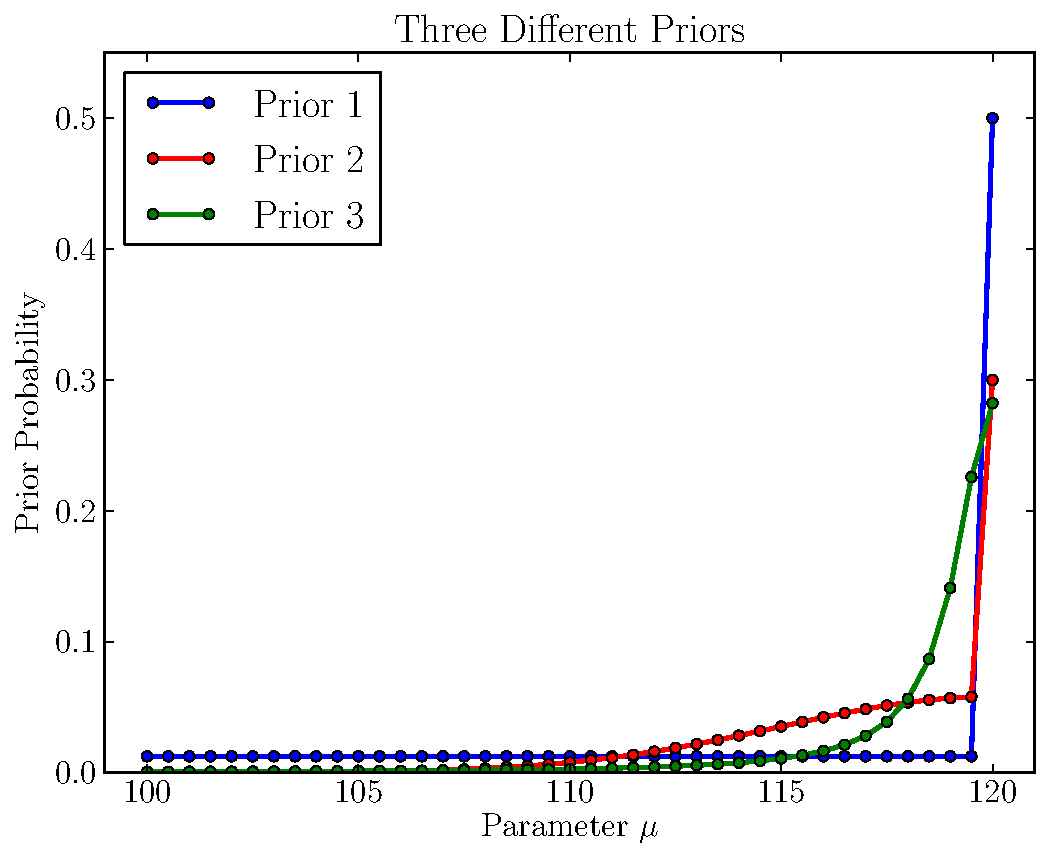
\includegraphics[scale=0.6]{Figures/testing_priors.pdf}
\caption{Three possible priors we could use for the blood pressure question.
All may seem ``reasonable'', and the choice can affect the results (quite
significantly in some cases). Care should be taken when choosing the prior
in hypothesis testing problems.
\label{fig:testing_priors}}
\end{center}
\end{figure}


\section{Some Terminology}
There is some alternative terminology that is widely used that is particular
popular in Bayesian hypothesis testing (aka model selection) problems. Suppose
there were two hypotheses $H_1$ and $H_2$, and some data $x$. Now $H_1$ and
$H_2$ might be a null and alternative hypothesis, or they might be two
particular values of the parameter, or whatever. Two repetitions of Bayes' rule
for these two hypotheses are:
\begin{eqnarray}
P(H_1 | x) &=& \frac{P(H_1)p(x|H_1)}{p(x)}\\
P(H_2 | x) &=& \frac{P(H_2)p(x|H_2)}{p(x)}
\end{eqnarray}
Dividing these two equations gives the {\it odds form} of Bayes' rule, which
deals with ratios of probabilities instead of probabilities themselves.
\begin{eqnarray}
\frac{P(H_1 | x)}{P(H_2|x)} &=& \frac{P(H_1)}{P(H_2)} \times
\frac{p(x|H_1)}{p(x|H_2)}\\
\end{eqnarray}





\section{Hypothesis Testing and the Marginal Likelihood}\label{sec:marginal_likelihood}


